\documentclass[sigconf]{acmart}

\input{format/i523}




\begin{document}
\title{Big Data Analytics in Product develop management}


\author{ZhiCheng Zhu}
\affiliation{%
  \institution{Indiana University Bloomington}
  \streetaddress{936 S Clarizz Blvd}
  \city{Bloomington} 
  \state{Indiana} 
  \postcode{47401}
}
\email{zhuzhic@iu.edu}


\begin{abstract}
    The success of a new product is to a large extent due to whether the producer making efficient and accurate strategies between the different stages of a product lifecycle. Big Data analytic techniques have the potential to improve the efficiency of product development, making accurate product strategy, channel strategy, pricing strategies and promotional strategies in the different period of a product lifecycle. In this project, I will try to figure out how the data affect the decision making and try to use the relation between different twitter account to describe the potential of the Big data also I will describe decision trees and PageRank and how do these tools produce a good market segmentation and market positioning for a product.
    
\end{abstract}

\keywords{i523, hid229, Big data, Product Development, Technology}

\maketitle

\section{Introduction: Big Data}
The advent of technology has resulted in virtually all industries and organizations collecting large volumes of data. The data collected results from diverse source, which include product sales, customer information, historical industry data, and employee information just to mention a few. Computers and the internet in particular have made it easier to collect data of different kinds because they make it easy to create, store, transfer, and analyze data. As a result, data has become a critical asset for many organizations and corporations in their bid to control the markets of the products or services they offer consumers. Furthermore, According to Arora, big data also refers to large and complex dataset (13). This means that it is virtually impossible to use traditional processing applications to organize and analyze this data. Therefore, there are various challenges associated with big data due to its large volume and complexity \cite{Arora2016}. These problems include data capture, data storage, data analysis, sharing of the data, making searches on the data and the privacy of the information \cite{Sivarajah2017}. Information increasingly becomes an important factor in determining the success of a product. A few years ago, manufacturing and the Internet have still belonged to two different separated industries, But as the mainstream consumer groups changed from old generation to Millennial generation, and the use of computers and the establishment and application of the Internet have produced a violent shock to the traditional way of product development, thus resulting in a new product development strategy. I have to say that the relation between the manufacturing and the Internet are getting closer and closer. One of the major changes might cause by using big data as a technique to develop right product and make effective promotion strategy.
\begin{figure}[!ht]
  \centering
\includegraphics[width=\columnwidth]{images/gain information.png}
  \caption{Difference between various generations \cite{gain1}}
  \label{Figure 3}
\end{figure}
\section{Examples of Big Data}
For example, organizations with an online presence such as online market places collect data from their clients. This includes different types of data such as customer information, purchases, and time spent on the website. For very large organizations (such as Amazon or eBay) dealing with thousands and probably millions of customers daily, this type of data soon becomes voluminous and difficult to analyze. For effective analysis, such data needs large physical storage space and organization in ways that will make it usable and of benefit to the organization \cite{Arora2016}. The main solution to this problem is the use of a data warehouses since traditional databases are too basic to handle the complexities involved with big data. Data warehouses provide the much-needed processing power needed in handling and analyzing big data \cite{Arora2016}.
Another issue is Outdated decisions and information are bound to create disadvantages when competing with other companies, but the traditional data processing system is obviously not suitable for the era of big data. Corporate decision-makers must adopt new technologies to face the changes of the times and customer. For example, Hadoop technology is a new and widely accepted technology.
\begin{itemize}

  \item ``Hadoop is an open-source software framework for storing data and running applications on clusters of commodity hardware. It provides massive storage for any kind of data, enormous processing power and the ability to handle virtually limitless concurrent tasks or jobs\cite{sas1}.''
\end{itemize}  
\begin{figure}[!ht]
  \centering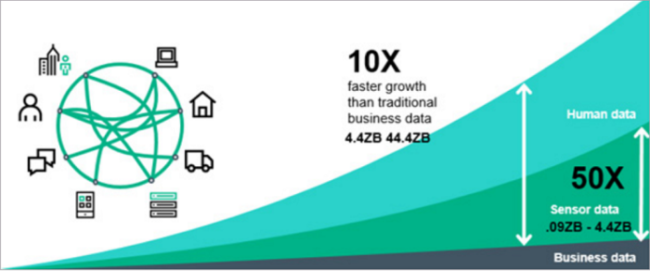
\includegraphics[width=\columnwidth]{images/data-growth-rate.png}
  \caption{The Exponential Growth of Data \cite{growth1}}
  \label{Figure 1}
\end{figure}
\subsection{Application of Big Data in Product Development}
how to clean the data and find useful data more quickly in product development is even more important.Quickly identify the characteristics of the target customers and their possible needs for a variety of products. base on the analysis, we can develop some products that more suitable for marketplace needs, or we can be more accurate when we try to find our potential target customer. According to different consumer behavior, we can design different software, for example, during the financial turmoil we found that lots of users are price sensitive, we can design a kind of software that can provide local discount merchandise information in real time.If the target customer is a group which wants higher quality of life, we can push more high value-added product.
One of the most vital areas where big data finds use is in product development management. The product development process allows for the design and release of new products into the market. Product development also involves processes such as forecasting, planning, and marketing of new products. The process adopted ensures that first the product developed meets a certain need in the market. Second, the process certifies that the price set reflects the amount consumers are willing to pay. Lastly, it guarantees the organization is making the product in such a way that it will be able to reach the targeted market. Typically, an organization will collect market data from various systems.

\begin{itemize}

  \item For instance, transaction-processing systems provide invaluable data to organizations \cite{Provost2013}. An example of a company that uses big data is the online market place Amazon. The market place has thousands of products stocked by the company and by third party sellers using the platform to sell their products. The checkout system in such an organization will collect very important data such as the products sold, the customers buying the products, the time of purchases and such details \cite{Walker2015}. The details of the customers will probably include the age and gender of the customer. When the company analyzes such data, it provides the management with a vital insight into the business’ activities and performance. Such as SEM analysis, SEM analysis is a research and analysis methods which focus on customer satisfaction. This is a good way to make a classification for our users. One of the most typical examples is some recommender systems such as Pandora use songs or artist properties to create a radio station, all of these songs and artist have similar attributes. User feedback is used to adjust the content of the radio and recommend some music which is more attractive to the listener.
\end{itemize}


\section{Analysis of Customer Needs and Market Demand}
\subsection{Anticipating Customer Needs for New Products}
For instance, using the data collected from the checkout system, the company can tell what type of products are likely to be bought and by which customers \cite{Walker2015}. Using information about customers contained in other systems such as customer relationship management (CRM) systems, the company can get information about the people likely to purchase a certain product, at what time they are likely to make the purchases, and the other goods they are likely to purchase with the products \cite{Walker2015}. The company can then use such information to make decisions on which products to stock, what price to sell them, which products to suggest to clients as they are making purchases and the time of day, week and even year that such products are in demand. For instance, Walker points out that big data plays an important role in helping Amazon launch new products. In particular, the data collected by the organization on books played a central part in the establishment of the Amazon Kindle product, which is highly successful in the market \cite{Walker2015}.
\subsection{Inventory Management}
Therefore, with the help of big data, product developers and manufacturers are able to ensure that the products needed by the customers are available in the right quantities and at the right times \cite{Davenport2014}. For example, a person purchasing a large flat screen television is also likely to purchase wall brackets for mounting the television set. The company can also get information on what brand and size of TV sets are in demand. The company can then ensure that it stocks such products when they are in demand. Because of the increased competition, profit margins can be very small. This requires the company to ensure efficiency to ensure that it avoids issues such as dead stock, which have negative impacts on profitability. Getting the right amount of products is critical as it ensures that the company meets all the demand and there are no excess items, which are a cost to the organization \cite{Provost2013}. 
\subsection{Anticipating Customer Demands}
\begin{figure}[!ht]
  \centering
\includegraphics[width=\columnwidth]{images/single hub node with high in-degree.png}
  \caption{Hub Node in network }
  \label{Figure 2}
\end{figure}
In addition, using big data, product developers able to anticipate demand for new products and it can therefore embark on developing such products and ensure that customers get the products. For example, Facebook the social media giant employs big data in making decisions on how to present its services for clients \cite{Morabito2015}. For instance, the company collects data on user activity on its platform \cite{Morabito2015}. Using this information, the company is able to present an interface customized to a specific user. Such data also finds use in targeted advertising, which is one of the key ways in which such companies make majority of their revenues. In 2013, Morabito pegs the revenue drawn by Facebook from advertising at almost  8 billion dollars \cite{Morabito2015}. The use of big data by the company has made it able to forecast the needs of the market and provide users with products and services that the customers find useful. This has resulted in the company becoming the world’s most used social media site and maintain its advantage over its rivals, some of which the company has ended up buying out. what is worth to mention is that some Big Data technique can help these company decide which user are more worthy of advertising. According to what I got from my programming, some people with a high degree centrality in their tweet network has a higher value than other people with a sparse network. Because the dense network can spread the information faster with a lower cost.



\section{Management of the Product Development Cycle}
In product development management, a product passes through various stages in the lifecycle. The main stages are product research and development stage, the introduction stage, the growth stage, maturity stage and the decline stage \cite{Stark2015}. Big data can help to ensure that a company develops a product that maximizes returns in each of the main stages. Once the product is in decline, the company also has the information needed to make decisions on the products it will introduce that will ensure that the company maintains its competitive advantage on the market. 
\subsection{Research and Development}
In the product research and development stage, an organization will collect large amounts of data from the public, from its own internal systems or data from third parties \cite{Ron2016}. Such data will contain information on the type of products favored by the market. The company will analyze this data and come up with information that its management can use to improve the overall decision-making process \cite{Ron2016}. 
Using the example of the online retailer Amazon, the company can use big data to carry out research and development processes to determine that many customers want an easier way of making payments. The organization can obtain such information directly from customers, as well as, based on received feedback. For example, the company could notice trends in customers who browse for items but abandon the purchase when they are required to pay. This may be because the payment methods offered by the company are difficult or customers are not confident in them. Using such information, the company can decide to introduce alternative ways to make payments, which are easy to use.
\subsection{Introduction Stage}
Big data also proves to be very useful in the introduction stage. For instance, a company selling warm winter clothes would not be successful is such items in summer. The main reason for this is that at the time, customers are not in need of the products. Organizations can derive such information by analyzing data on the type of purchases made by customers in different periods of the year.
\subsection{Growth Stage}
Furthermore, the growth stage is also vital for any product in the market. During this stage, the product introduced by the company gains a foothold in the market \cite{Stark2015}. During this stage, more and more customers learn about the product and they are likely to make a purchase. Using big data can be advantageous to a company as it can help it to organize its marketing appropriately. The purpose of this is to ensure that the products reach the widest coverage \cite{Ron2016}. Big data can also help the company in making decisions such as which locations to introduce the product.
\subsection{Maturity Stage}
Similarly, in the maturity stage of the life cycle of a product, the product has already gained a foothold in the market and its growth slows down \cite{Stark2015}. Big data can help the company to make decisions that will enable the product to maintain growth during this stage for the longest time.
\subsection{Decline Stage}
The decline stage occurs after a product has been in the market for a while and probably newer technologies have become available reducing the usefulness of the product to the market \cite{Louis2013}. Big data can help the organization in this stage of the product life cycle by ensuring that the product remains available for people who still need the product. For example, smartphone use has overtaken the use of feature phones in the market. Feature phones offering simple functions have therefore reached the decline stage of the cycle. Despite the noted decline in the global environment, in many developing countries feature phones remain in demand due to factors such as battery life and cost. Using big data, a company manufacturing feature phones can understand its market and therefore be able to ensure that supply to such markets remains available. 
Moreover, by the decline stage of the product life cycle, the company dealing with the product is likely to have begun the research into the next product that it will offer to clients that will meet their emerging needs. Big data, which will consist of data collected from the lifecycle of the previous product, will prove to be very useful in the development of the new product. As the name suggests, this is a lifecycle and the process should ideally continue indefinitely for the company. This ensures that the company is always ready with a new product that is able to meet the demand of clients in the market. 
Constant innovation is vital in the modern market where competition is very high. Nokia Corporation, once the largest manufacturer of cell phones is an example of a company that failed because of not innovating constantly. In the mid-2000s when competing firms introduced the first smartphones, Nokia was the dominant player According to Robbins, Rolf, Ian, and Mary by 2007 Nokia controlled 40 percent of the global mobile phone market \cite{Louis2013}. However, because of poor forecasting, the company continued to manufacture its previous phones and soon it lost its market share to other companies manufacturing smartphones such as Apple \cite{Robbins2014}. The use of big data in making decisions during the product lifecycle can help a company to avoid making such mistakes, which may prove to be catastrophic. 
From the analysis above, it is evident that during the different stages of the product lifecycle, there are different strategies that organizations can employ. For example, product manufacturers and sellers can utilize different marketing strategies during the different stages of a product’s lifecycle. The marketing strategy that is useful in the introduction stage may not be as effective during the growth stage of the product. The production strategy employed during the introduction stage may be very effective but the same strategy when employed during the growth stage or other subsequent stages may not be very effective. Big data therefore helps an organization to make the best decisions on different strategies based on the information obtained from analyzing the data. This ensures that the strategies selected for various activities during the different stages of the product’s life are the most appropriate which ensures that the company is able to gain the most benefits from its products. 
\section{Big Data Analysis Methods}
In big data, organizations can adopt different analytic methods in order to extract useful information. Data in its raw form is not very useful to an organization. Analysis of the data ensures organizations come up with patterns emerging in the data with the aim of improving the decision making process. The analytical method chosen for analysis of big data depends on various factor such as the type of data available (e.g. qualitative or quantitative), the amount of data available and the result desired. Among the most common analysis methods in big data are Decision tree analysis, PageRank, and kNN algorithm.

\subsection{The Decision Tree Analysis}
The decision tree analysis is a method of analyzing data that uses a graph in the shape of a tree, hence the name. In this method of analysis, a decision maker considers a decision and its resulting consequences \cite{Zhang2015}. These consequences include the chance of the consequence occurring, the costs involved when the consequence occurs and how useful the consequence is for the organization. The initial decision represents a node and the possible consequences are the branches \cite{Guller2015}. Each consequence then becomes another node and the tree represents consequences in further branches \cite{Guller2015}. When using a decision tree to make a decision, the decision maker selects the path that is most likely to lead to the desired solution. Big data requires the analysis of large amounts of data. A decision tree algorithm will analyze the data available and present a decision tree with all the possible paths (the connections between nodes and branches) based on the information available \cite{Guller2015}. 
For example, the decision to select a particular marketing strategy will show the chance of it achieving the result, the costs involved, and the utility to the company, depending on the information obtained from the large data sets. This will therefore present different paths based on the different strategies chosen. Usually, the decision maker will make a decision by selecting the path of least resistance. Usually this path contains the best attributes needed by the organization. For instance, one path may be more costly than a different path based on the strategy chosen but they eventually lead to the same result. The path that costs less will therefore be best suited for the organization since it will allow it to achieve its objective more efficiently. Lastly, because making a decision will lead to different consequences (which in themselves require other decision) the path that best suits the organization results from the final objective through the path of branches and nodes that best meet the needs of the organization \cite{Guller2015}.

\subsection{PageRank}
PageRank is an algorithm named after Larry Page who was a co-founder of the search giant and technology company Google. This algorithm finds use in ranking the search results on the search site \cite{Zomaya2017}. This algorithm works by counting the number and quality of links to a webpage. This algorithm helps to determine the quality of the information on the different WebPages with information related to the search queries entered \cite{Langville2006}. Based on the quality and number of links pointing to a page, the algorithm is able to determine the quality of the webpage \cite{Zomaya2017}. This then results in the page receiving higher raking in search results. PageRank is very important as it helps the search giant to present the most relevant answers to queries made on its site. 

For instance, one webpage may contain very many links concerning the search query but the information contained on the webpage may not be of the highest quality. This means that another webpage with higher quality information even with fewer links can still rank higher than the other webpage \cite{Langville2006}. This algorithm works by using data generated from previous searches with similar queries. Such an algorithm makes extensive use of big data to ensure that it presents the most appropriate results for a person making a query. 


\subsection{k-NN algorithm}
The k-NN algorithm is an algorithm used in pattern recognition \cite{Yingmin2017}. It finds use in both classification and regression. This is the simplest form of machine learning as it uses an approximation of values nearest to the value under analysis. For instance, in classification, the desired output is class membership. The algorithm achieves this by looking at the nearest neighbors of the value under inspection. The value receives assignment to the class to which most of its nearest neighbors belong. In regression, the desired output is typically the property value of the object under study. This is obtained by getting an average of the values of the objects that are the immediate neighbors of the object being inspected. This means that the nearest neighbors to an object contribute more towards its value than objects that are located further away from the object inspected. This means that using these algorithms, the values of an object can be predicted accurately, which helps in making complex decisions easier based on the immediate results expected \cite{Yingmin2017}.

\section{Big Data Analytics and Decision Making}
\subsection{Big Data and Competitive Advantage}
Data as previously mentioned is one of the most important assets for any business. This data needs to be analyzed so as to come up with usable information that help the management of the organization to make decisions that are likely to succeed in the market. Because of the increased competition in the modern business environment, many organizations have employed big data to help them make decisions such as how to arrange items in stores, what items to stock, the prices that are best for the market and such decisions \cite{Walker2015}. Although these decisions might look simple, it is very important for an organization to get them correct. Miscalculations made in such decisions could lead to losses including financial and market share losses. This is because modern customers want value for their money. This means that the organization must offer the best possible services at the lowest cost. 
Furthermore, this makes them attract more customers for their products or services and in the process enable them to make a higher margin. Because most competitors will use some form of data to make their decisions, it is very easy for an organization or company to lose its competitive advantage to its competitors \cite{Walker2015}. Many organizations consider making accurate decisions in an efficient way a critical aspect of their competitive advantage. For instance, a company can release a product before the competition releases their version. Customers will buy the product already in the market allowing the organization to gain a market advantage over the rivals who have not released their product. Big data has made it possible for such organizations to obtain patterns from extremely large data sets, which are more accurate and therefore likely to produce accurate decisions \cite{Walker2015}.
Another strategy can help our product to attract more customers is using the internet hub node to spread the information about our product and advertising on the network, the network hub node is a node with a number of links that greatly exceeds the average. for example, Donald Trump's twitter is one of a most popular node in twitter network. If someone can lobby Trump to promote the product I believe we will have increasingly more customer growth. These hubs play the same role such as what Macy's used to play. Macy's used to be a big node for people's Holiday purchase. because it attracts most of the people living in that area to enter the store. The famous twitter account attract their follower because they have a fancy lifestyle or fulfill some value their follower admired. all of these are helpful for product promotion and the spread will have a more incredible efficiency and effectiveness.

\section{Conclusion}
In conclusion, despite the use of big data already being widespread in the business world, its importance will continue to grow with time. This is because of the large number of devices that are now generating data. The internet of things has resulted in a situation where even everyday appliances connect to the internet and they have the ability to collect large amounts of data. This results in more data that organizations can analyze to discover patterns in the market that organizations can exploit. Organizations are also overcoming the challenges facing big data with the collection of data now largely automated from different systems internal and external to the organization. 
Moreover, specialty companies have come up with the sole purpose of collecting and analyzing market data. Manufacturers are offering solutions to the technological challenges involved in big data by developing larger storage devices that are able to store increasing amounts of data efficiently. The security of such information has seen significant improvements with more secure communication and storage channels. The use of big data is also set to increase as current analytic methods become efficient. New analytic methods are also likely to be developed that will ensure that the data collected from independent systems and the market are analyzed better in order to develop information that can be acted upon more readily in the market. This point to a future where big data will be more important than ever in ensuring that companies come up with products and strategies that enable them to be more competitive in the market and therefore increase their chances of survival in the market.





\begin{acks}

  The authors would like to thank Dr. Gregor von Laszewski for his support and suggestions to write this paper as well as TAs' helpful suggestions on this paper.. 

\end{acks}

\bibliographystyle{ACM-Reference-Format}
\bibliography{report} 

\end{document}
